\section{Shared memory parallelisation}
\label{section:shared-memory}

We introduce three levels of shared memory parallelisation on a single machine that exploit multiple levels of locality. The hierarchical categorisation of the methods is based upon the abstract algorithmic distance between shared resource parallel utilisation and actual arithmetic computation. At the highest level we exploit  data access independence of vertex touches we assign cell block tasks to threads. Within each vertex touch particle pairs are grouped into aligned memory blocks thus tasks are launched between particle-to-particle comparisons. Lastly within each particle pair at the innermost level tessellation elements of the mesh are dichotomised and parallel locality is held for the underlying vectorized contact solver.

Three levels of multicore parallelisation:\\

a) cell level cell-to-cell thread units\\

b) cell vertex level particle-to-particle thread units\\

c) particle level mesh-to-mesh thread units\\

%describe the setup
We utilise particles approximated by a random spherical point cloud, arbitrary particle surfaces are generated with the Delauny triangulation algorithm. The algorithm is scaled in three respects; number of non-spherical particles, irregularity of particle radius size, and mesh size. Respectively, we provide three parameters in the creation of the simulation domain. $Rmin$, $Rmax$ parameter for max and min radius of particles, $m$ for mesh density, $p$ for number of particles in the domain. These allow observation of the interplay between performance and particle geometry and dynamics within a grid in a modern NUMA architecture. For scaling measuring we use the hybrid and the brute force solvers.

%Initial-termination conditions
For the experiment the initial space configuration of the particles in respect to the grid is homogeneous and aligned per cell. Initial conditions for the particle dynamics are governed by only gravity and termination is defined by the number of iteration that the granulates are rest condition with energy dissipated on the ground. Termination phase is known a priori. We utilise regular grid and reluctant-adaptive grids for space decomposition and and grid adaptivity to granular kinematics. 

\iffalse
\begin{figure}[htb]
	\centering
	\begin{subfigure}{.5\textwidth}
  		\centering
    	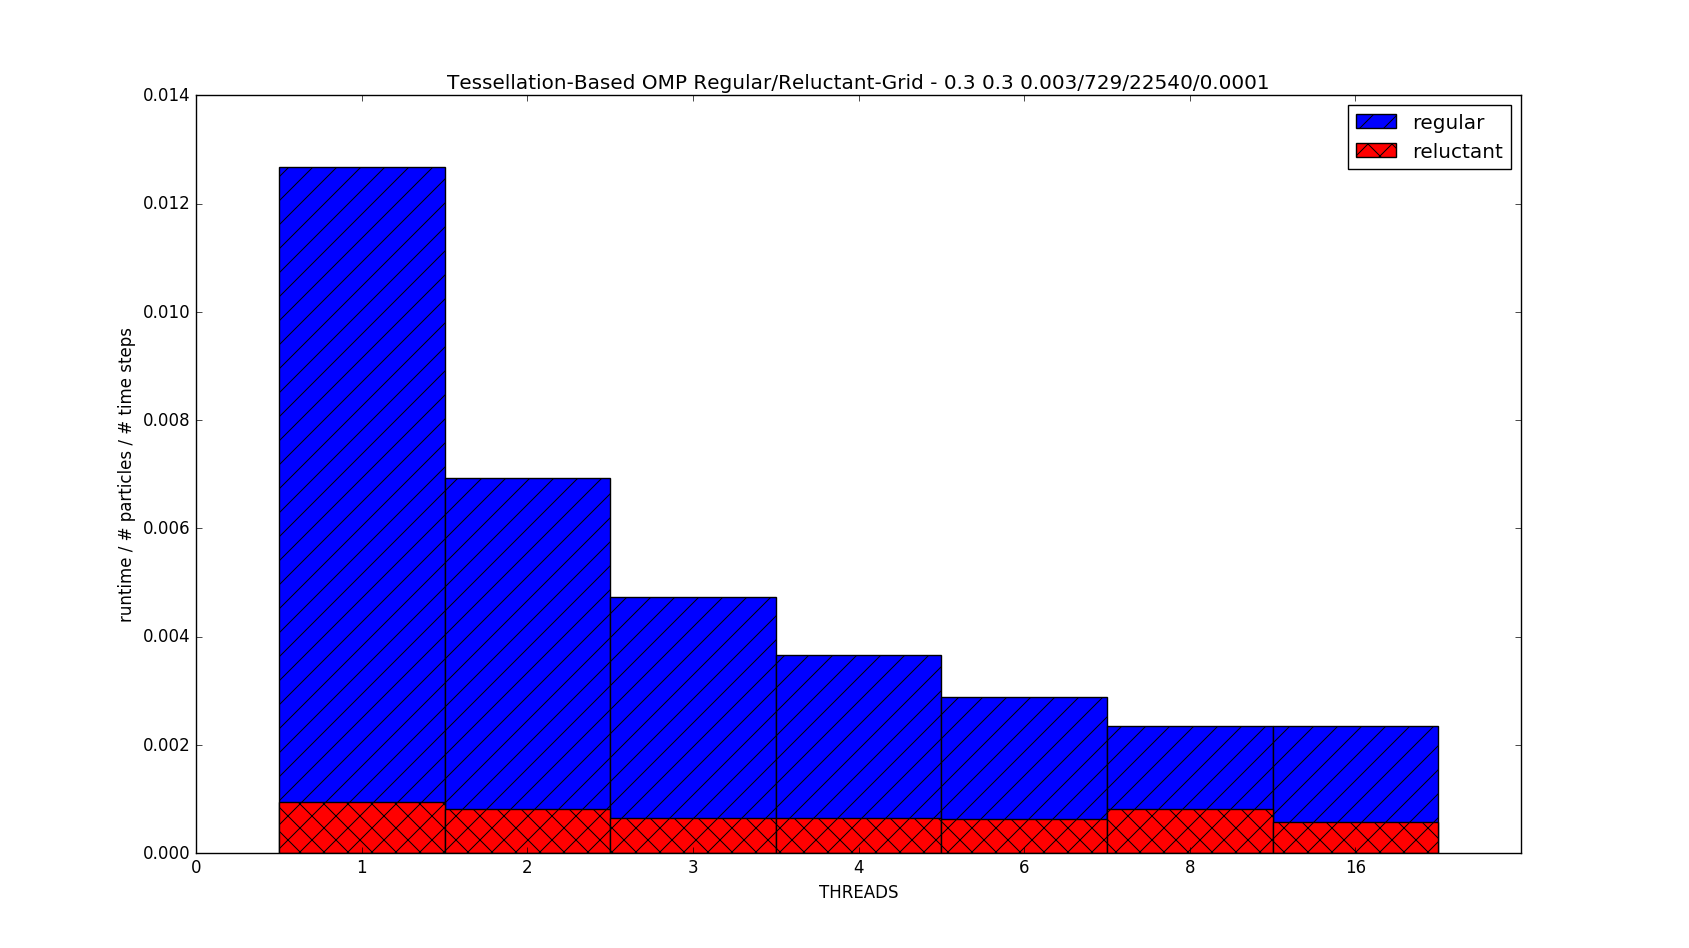
\includegraphics[width=1\textwidth]{experiments/omp/omp_mesh_regular-reluctant_20.png}
  		\caption{Shared memory scaling 22540 elements.}
  		\label{figure:omp_regular_reluctant_triangle_200}
	\end{subfigure}%
	\begin{subfigure}{0.5\textwidth}
  		\centering
    	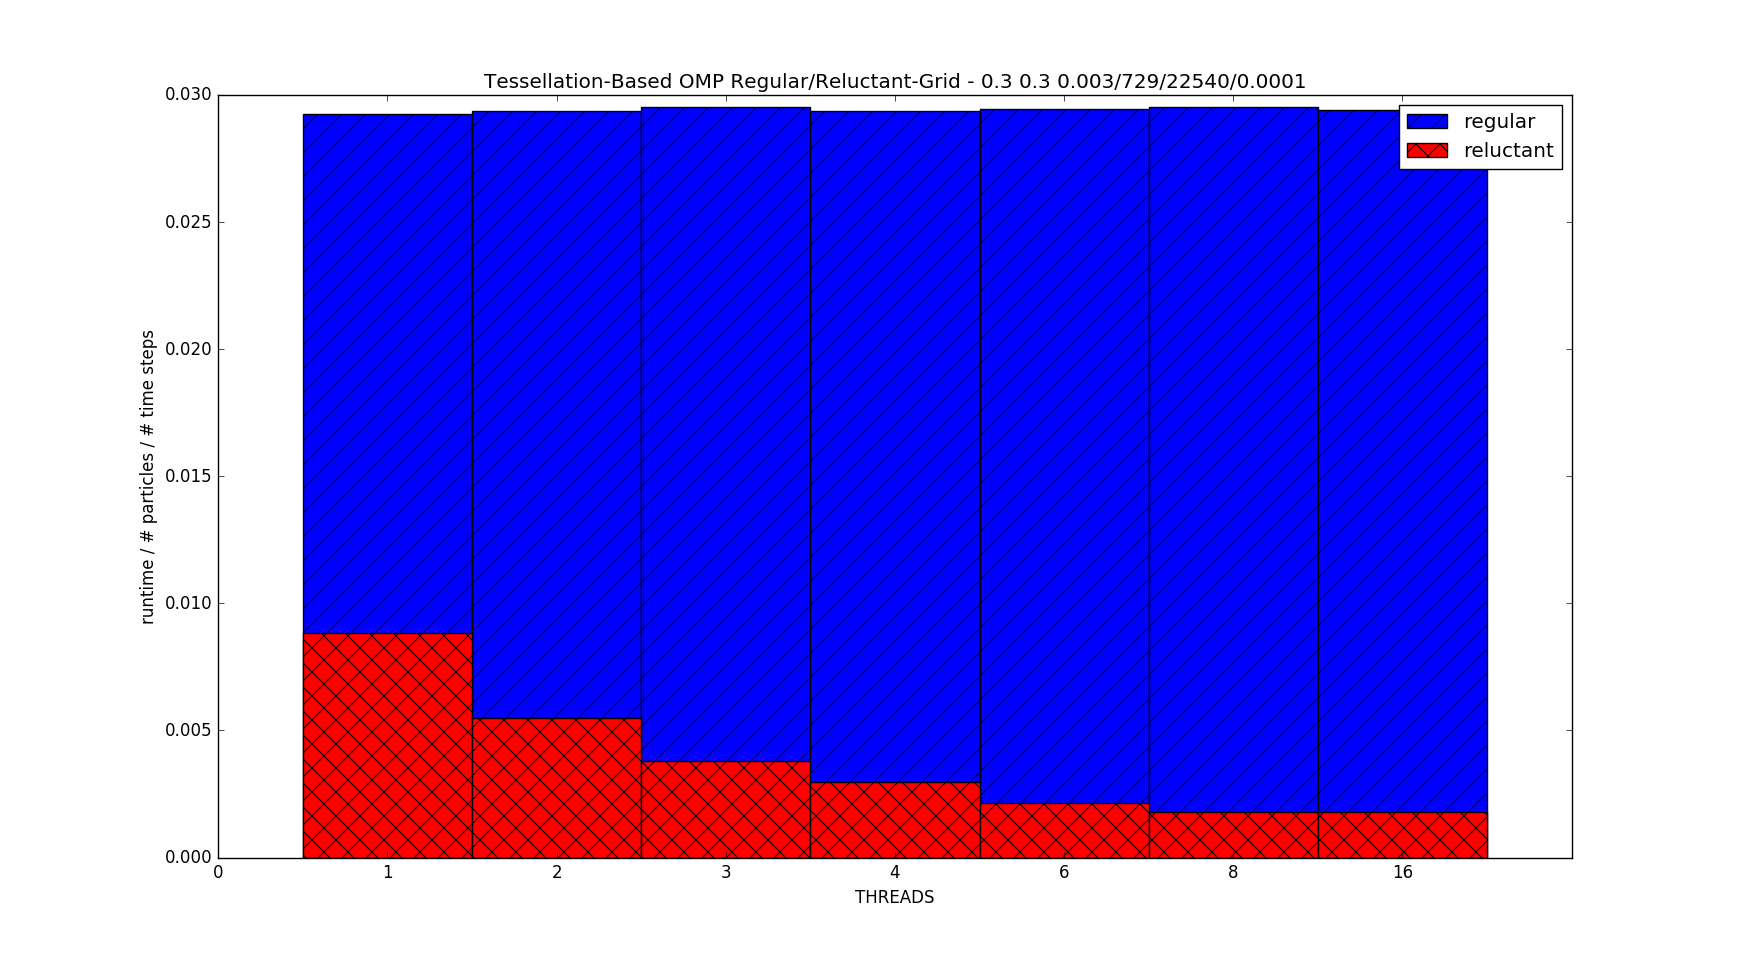
\includegraphics[width=1\textwidth]{experiments/omp/omp_mesh_regular-reluctant_200.png}
  		\caption{Shared memory scaling 98540  elements.}	
  		\label{figure:omp_regular_reluctant_triangle_200}
	\end{subfigure}
\end{figure}
\fi

\begin{figure}[htb]
  \begin{center}
    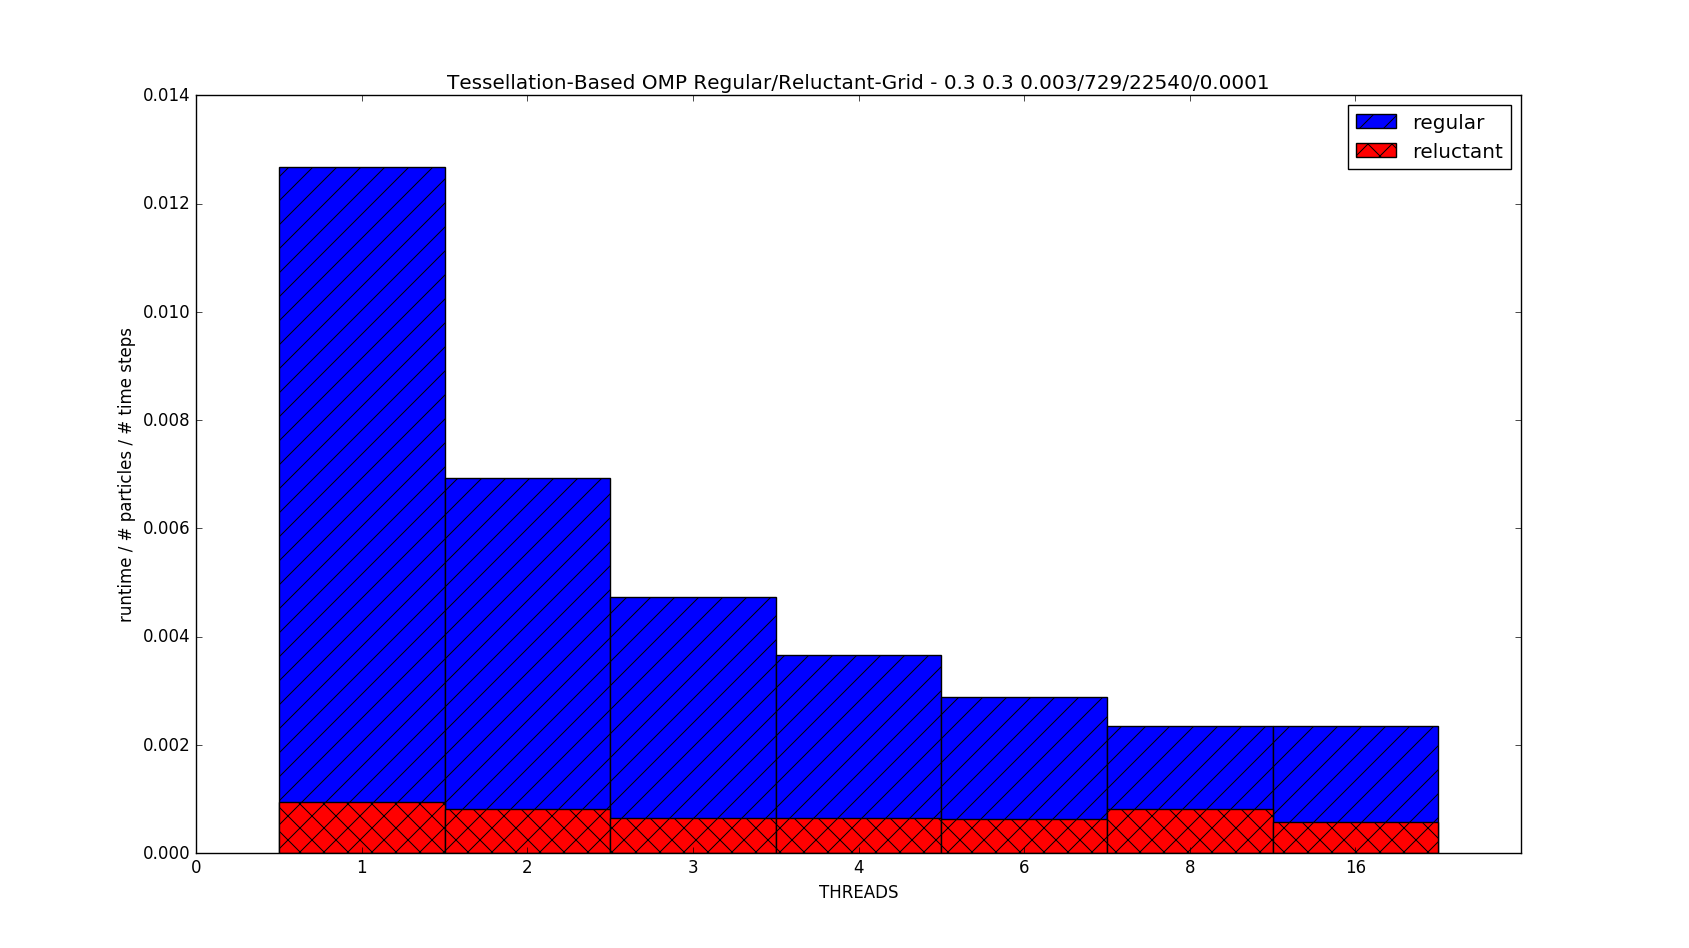
\includegraphics[width=1\textwidth]{experiments/omp/omp_mesh_regular-reluctant_20.png}
  \end{center}
  \caption{Grids shared memory scaling 22540 triangle elements (BF solver).}
  \label{figure:omp_regular_reluctant_triangle_20}
\end{figure}

\begin{figure}[htb]
  \begin{center}
    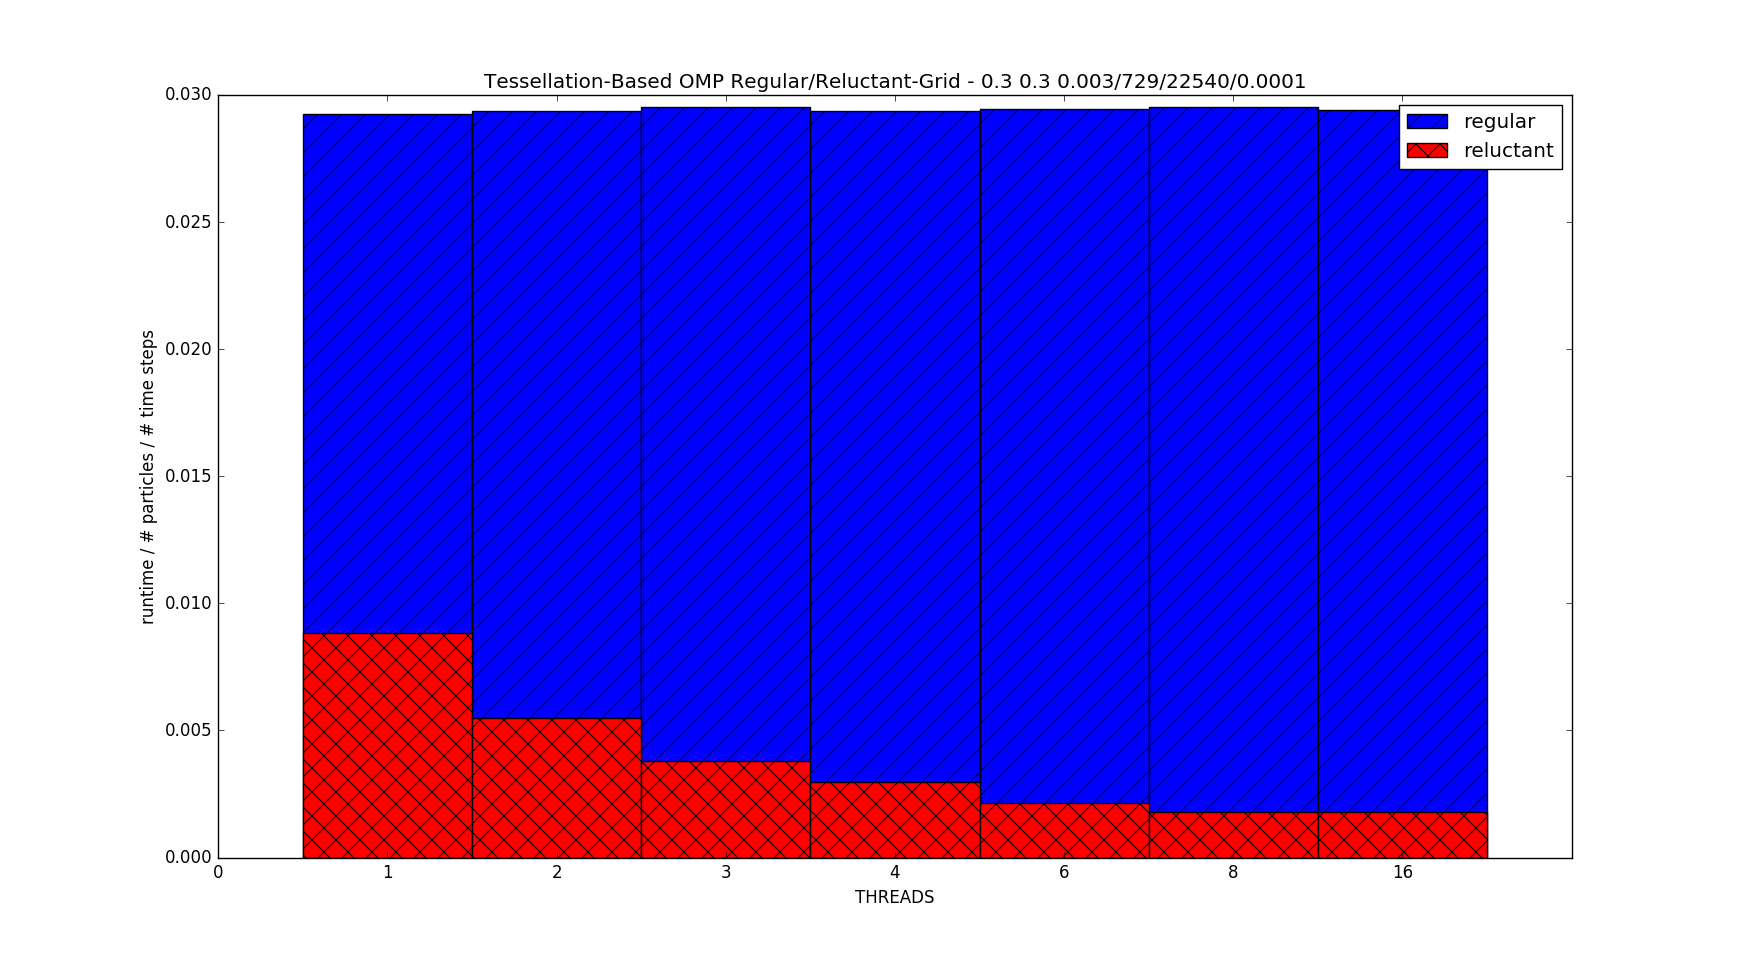
\includegraphics[width=1\textwidth]{experiments/omp/omp_mesh_regular-reluctant_200.png}
  \end{center}
  \caption{Grids shared memory scaling 98540 triangle elements (BF solver).}
  \label{figure:omp_regular_reluctant_triangle_200}
\end{figure}


%STEP A
Beginning at the innermost tessellation-level with a regular grid (figure \ref{omp_regular_reluctant_triangle_20}) on a NUMA ivy bridge system the code scales linearly up to the eight-core single die. As the size of the problem increase for weak scaling (figure \ref{omp_regular_reluctant_triangle_200}) the computation to memory bandwidth rate ratio is no longer sustainable computation to scale over multiple cores. Similarly on a small computational domain (figure \ref{omp_regular_reluctant_triangle_20}, blue) with minimum weighted threads grid adaptivity doesn't pay off as thread initialisation, scheduling, grid adaptivity and memory access overhead dominates over arithmetic intensity. Contrary to regular grid, adaptivity allows up-scaling towards both increasingly larger computations (figure \ref{omp_regular_reluctant_triangle_200}) and number of cores as long as bandwidth, compute bounds are not reached or thread overheads are not the bottleneck. In all cases the brute force solver does not scale pass the second die interconnect as communication to memory stagnates.

\begin{figure}[htb]
  \begin{center}
    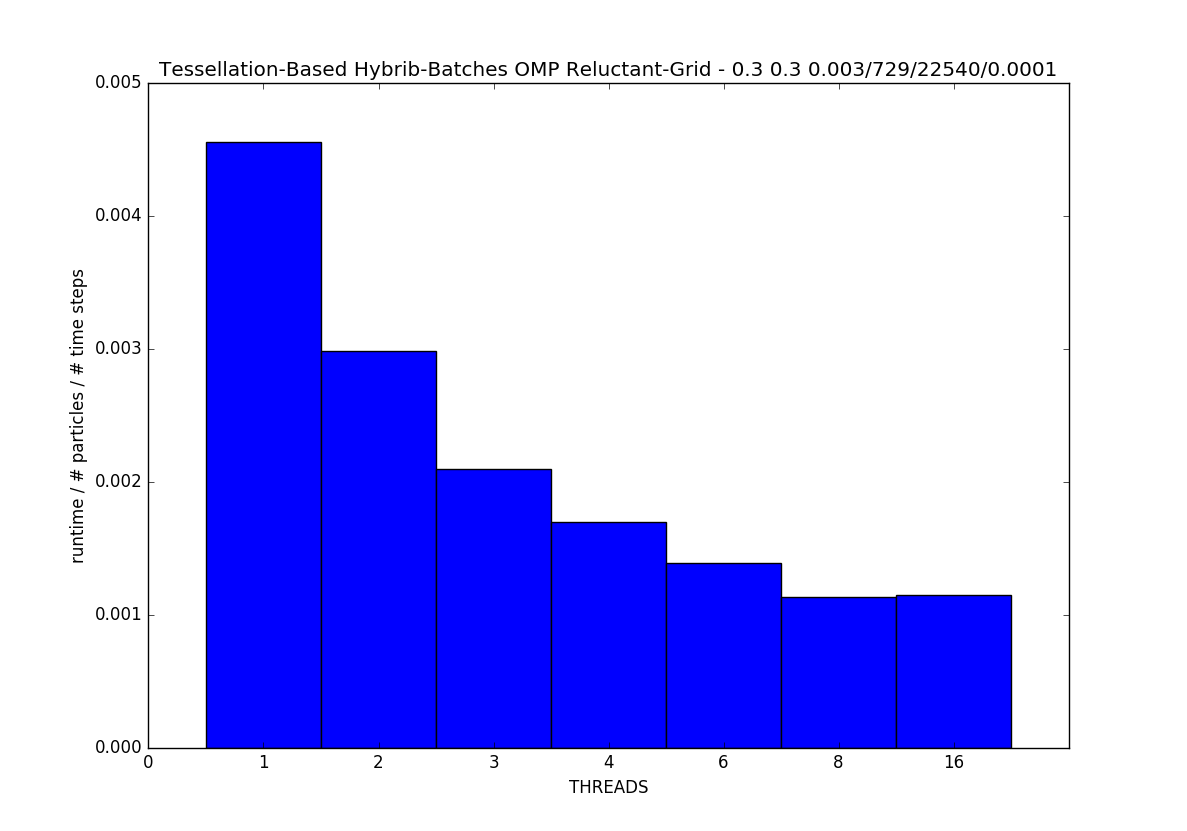
\includegraphics[width=0.8\textwidth]{experiments/omp/hbatches_omp_triangles_200.png}
  \end{center}
  \caption{Triangle based shared memory running hybrid-on-batches (HBatches).}
  \label{figure:hbatches_triangles_triangle_omp}
\end{figure}

Arithmetic, bandwidth intensity and data access patterns vary among solvers in the innermost level and can yield different performance results. The hybrid solver is parallelised in two different hybrid schemes triangle-to-triangle pairs and triangle-to-triangle batches, both launch different types of threads. For the hybrid-on-batches solver the tessellation-based threads
are $n$ triangle batches wide while hybrid-on-triangles solver relies on fine couples of threads. The non-deterministic nature and error-prone distribution of triangles of the hybrid algorithm as discussed in Chapter {-hybrid chapter-} would suggest that alternative scheduling would pay off. But for our experiments dynamic and guided thread scheduling don't have a performance gain but they rather create scheduling overhead due to error distribution in triangle pairs and due to the granularity of our batches. For the hybrid-on-triangles that is also the case because although the arithmetic intensity is dense in the solver, it doesn't last long enough to significantly overlap the cost of threading overhead. 

\begin{figure}[htb]
  \begin{center}
    \includegraphics[width=0.8\textwidth]{experiments/omp/
htriangle_omp_triangles_200.png}
  \end{center}
  \caption{Triangle based shared memory running hybrid-on-triangle-pairs (HTriangles)}
  \label{figure:htriangles_triangles_triangle_omp}
\end{figure}


\begin{figure}[htb]
  \begin{center}
    \includegraphics[width=0.8\textwidth]{experiments/omp/
bf_vs_hbatches_omp_200.png}
  \end{center}
  \caption{Triangle based shared memory running hybrid-on-triangle-pairs (HTriangles)}
  \label{figure:bfvshbatches_triangle_omp}
\end{figure}

Figure \ref{figure:hbatches_htriangles_triangle_omp} hybrid-on-triangle and hybrid-on-batches scales up to eight cores on the single dice but also neither gain from offloading to the second socket. In practice hybrids normalized time to solution is significantly greater than brute force as seen in Figure \ref{bfvshbatches_triangle_omp}

%VITUNE results and memory bandwidth compared to stream.  

%STEP B

At the outer parallel blocks, particle blocks are threaded within each grid-vertex touch. In Figure \ref{figure:particle_omp} brute force does not scale at all and that is due to the adaptive domain decomposition and not due to the solver. The aggressive particle decomposition per grid cell since the preconditioning of the simulation creates a access pattern contradiction to the dense tile access patterns that tessellation method exploits. The overhead and the precondition enforced by the grid for minimum number of particles per vertex doesn't allow any scaling to occur on any method. Particle density is too low for thread launching and compute-wise scaling, memory communication overtakes the simulation time. 

\begin{figure}[htb]
  \begin{center}
    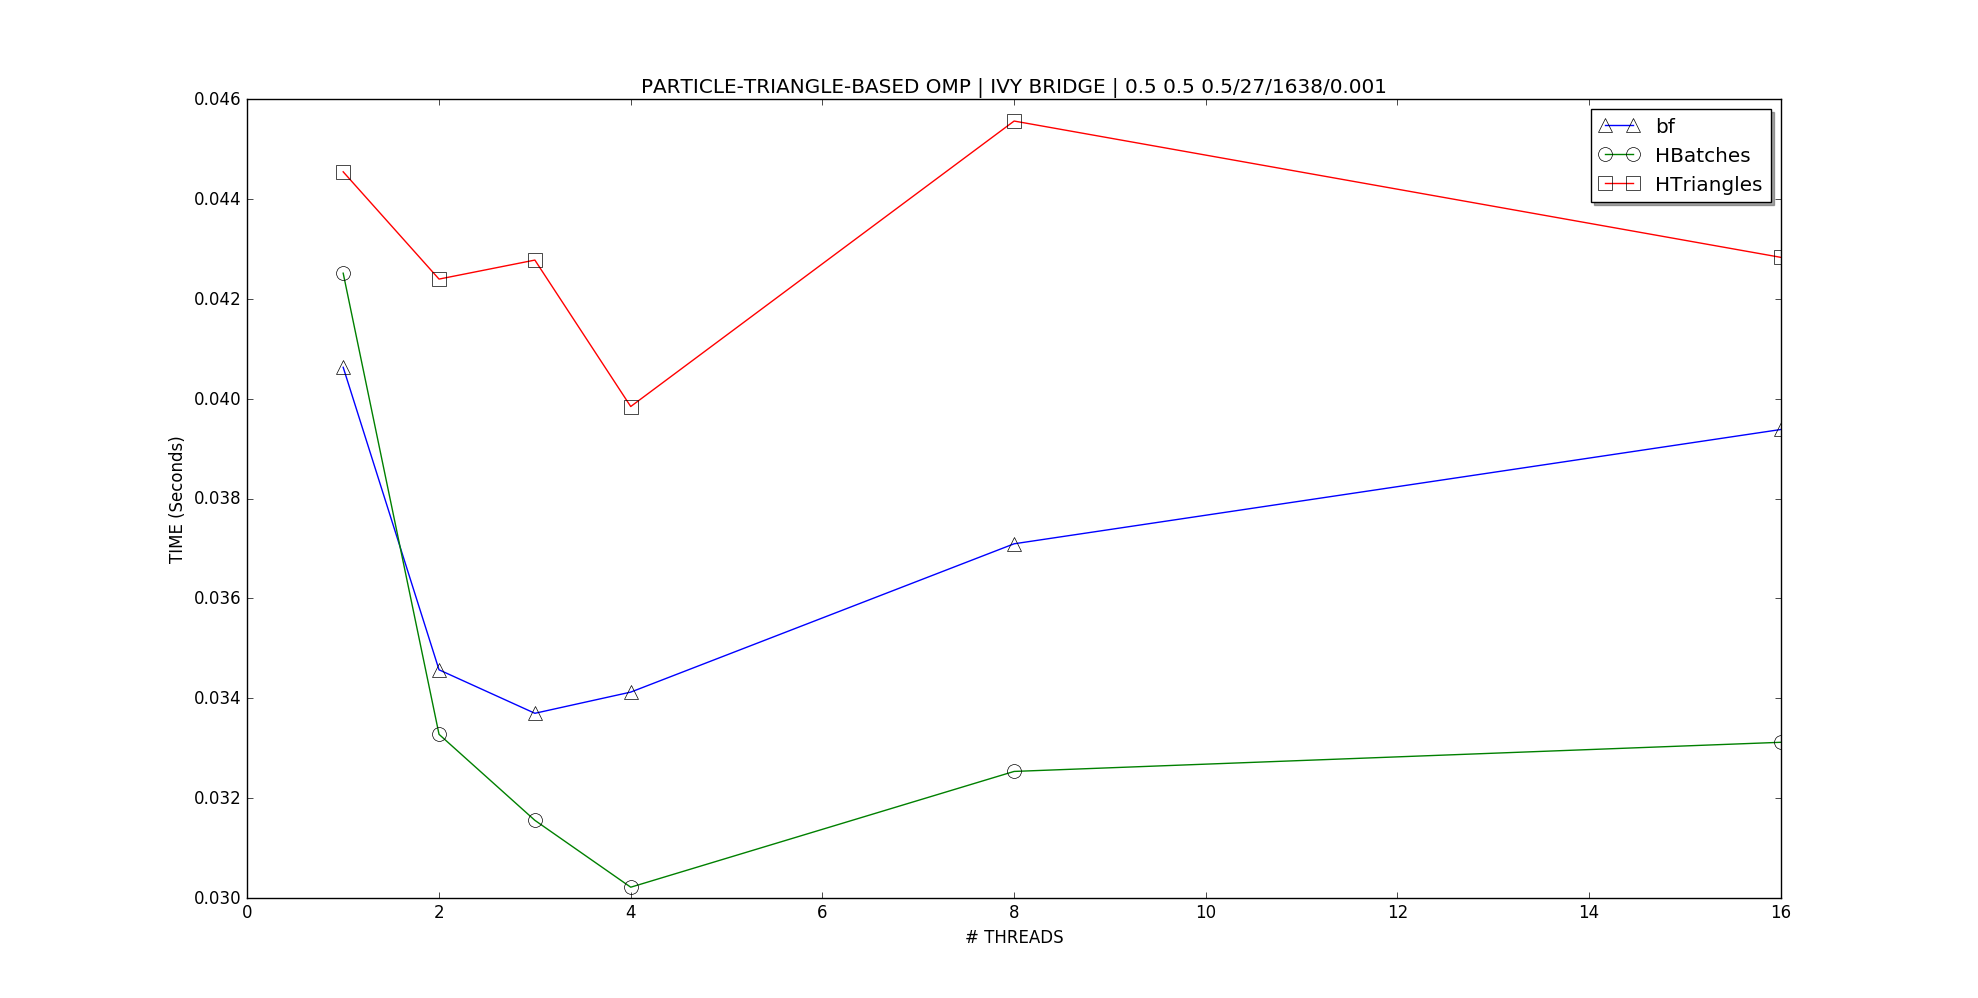
\includegraphics[width=1\textwidth]{experiments/random/omp/particle_triangle_based_x0.png}
  \end{center}
  \caption{Particle based nested shared memory brute force (bf)}
  \label{figure:particletriangle_omp}
\end{figure}

%Particle and Triangle parallelism nests both particle and triangle shared memory threads. The runtime to solution is slightly slower than particle-based parallelism due to overhead. 

%Nevertheless it has an impact on brute-force method as it scales smoother than particle-based only parallelism due to overhead. In this case hybrid-on-batches is also the fastest while the hybrid-on-triangle-pairs the slowest. 


%STEP C

\begin{figure}[htb]
  \begin{center}
    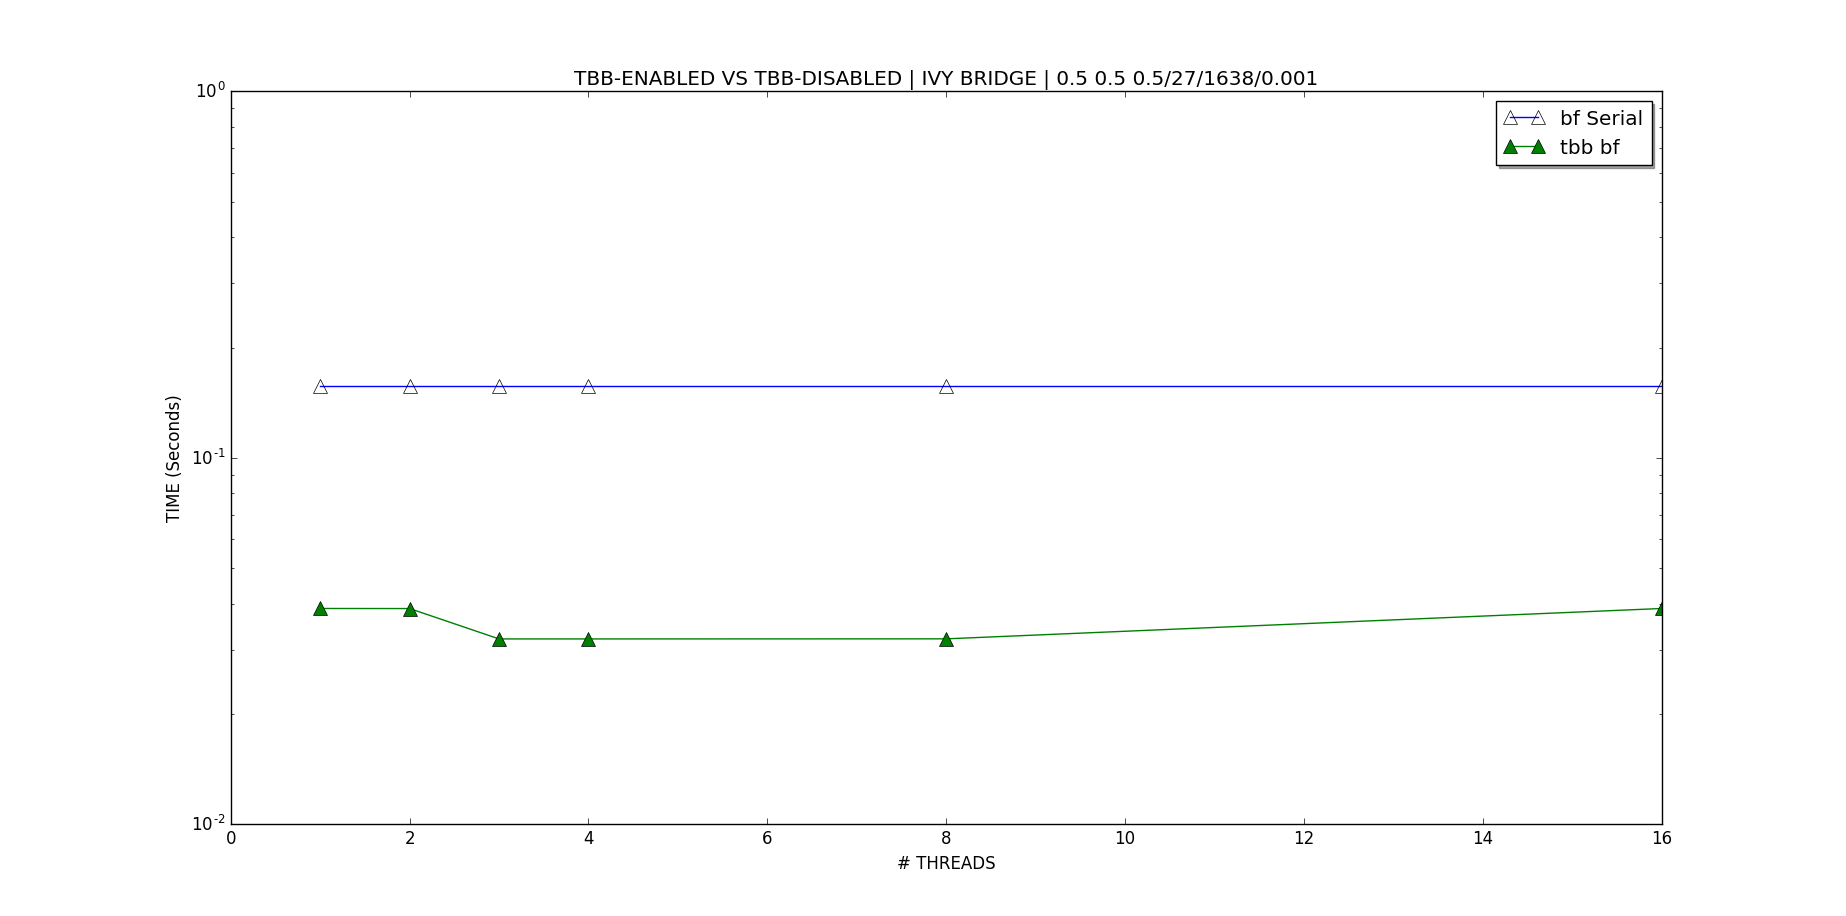
\includegraphics[width=1\textwidth]{experiments/random/omp/tbb_vs_serial.png}
  \end{center}
  \caption{Cell based parallelism on Peano compared to serial runs using Intel TBB}
  \label{figure:tbb_vs_serial}
\end{figure}
  

At the highest level of shared memory parallelism is the grid cell-based multicore processing. It is based on the peano-framework that is using Intel TBBs to assign cells on threads. This has significant impact on the overall runtime performance in Figure \ref{figure:tbb_vs_serial} it is compared with plain serial execution. Number of threads on the x axis refer to TBB Cell-based threads, at the contact detection method level the computation is performed without shared memory parallelism but with vectorization enabled. For the specified experiment in Figure {} we observe no cell-based thread scaling but only reduction of time to solution. But when we increase the problem size further (figure \ref{figure:tbb_scaling}) we see that cell-based parallelism scales and it enhances execution time. 

\begin{figure}[htb]
  \begin{center}
    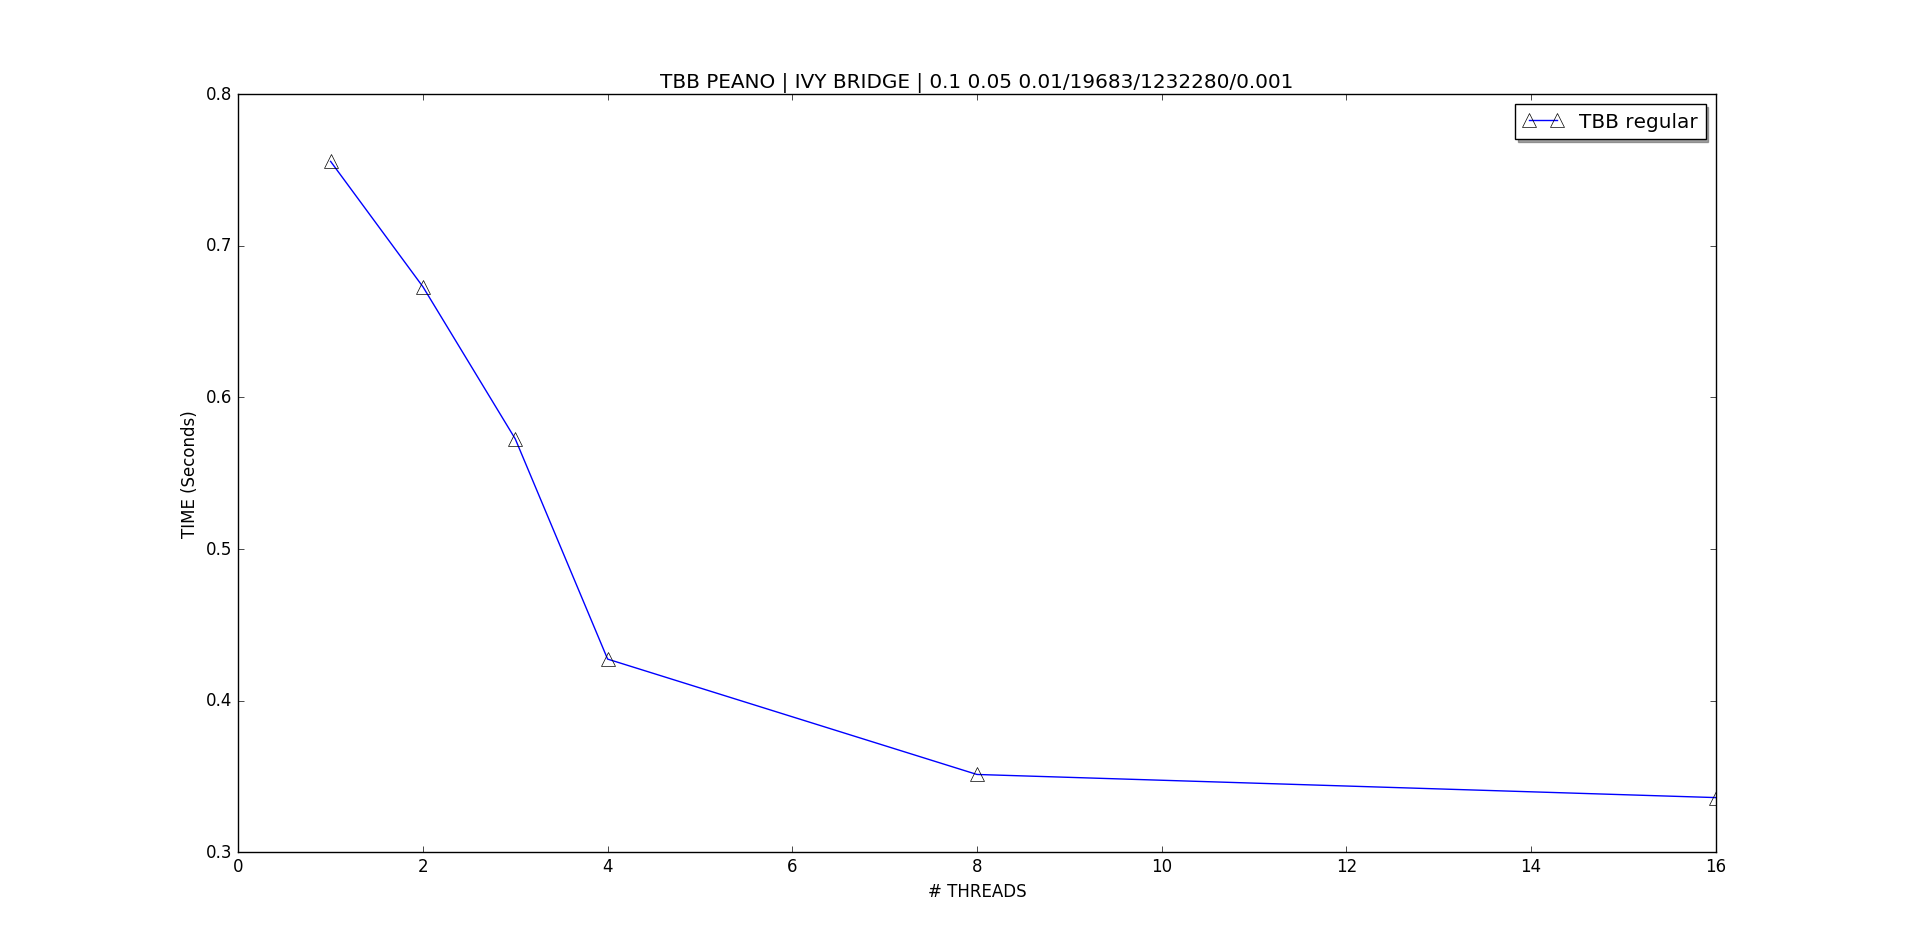
\includegraphics[width=0.8\textwidth]{experiments/random/omp/tbb_regular_x2.png}
  \end{center}
  \caption{Cell based parallelism on Peano compared to serial runs using Intel TBB}
  \label{figure:tbb_scaling}
\end{figure}

Overall shared memory parallelisation yield good speed ups both for hybrid and brute force using adaptive grids with triangle-based parallelism show good time-to-solution For large problem sizes the combination of cell-based plus triangle-based parallelism using hybrid-on-batches is the preferred option. Additional speedup can be gained if spheres are used as a filtering bounding box stage to our triangle-to-triangle contact detection.

\clearpage

